\documentclass[11pt, a4paper]{article}
%\documentclass[11pt, a4paper]{report}
\usepackage[utf8]{inputenc}
\usepackage{hyperref}
\usepackage{setspace}
    \onehalfspacing % set document spacing to 1.5
\usepackage[australian, english]{babel} % australian used to format date
\usepackage{amsmath} % for \eqref to reference equations
\usepackage{graphicx} % for inserting figures
\usepackage{url}
\usepackage{parskip} % no paragraph indentation, better indentation
\usepackage[left=1.5in, right=1in, top=1in, bottom=1in, showframe]{geometry}
%\usepackage[document]{ragged2e} % for easier justification of text
%\usepackage[nottoc]{tocbibind}
%\usepackage{booktabs} % more professional looking tables
\usepackage{blindtext}

\renewcommand{\thesection}{\arabic{section}} % remove chapter numbers from section numbers
\addto{\captionsenglish}{\renewcommand{\bibname}{References}} % rename bibliography

\begin{document}
\pagenumbering{roman}

% Front matter
\begin{singlespacing}
    % Title page
    \begin{centering}
        {\LARGE University of Waterloo} \\
        {\large Faculty of Engineering} \\
        {\large Department of Electrical and Computer Engineering} \\
        \vspace{5cm}
        {\Huge Title of Report} \\
        {\Large Self-study} \\
        \vfill
        Prepared by \\
        Dale Martin \\
        20573932 \\
        d2martin@edu.uwaterloo.ca \\
        4A Electrical Engineering \\
        \vspace{0.5cm}
        \begin{otherlanguage}{australian}
            \today \par
        \end{otherlanguage}
        \thispagestyle{empty} % suppress page number showing on this page
    \end{centering}
    
    % Letter of acceptance
    \pagebreak
    \begin{raggedright}
        Dale Martin \\
        5-514 Quiet Place \\
        Waterloo, Ontario, Canada \\
        N2L 5A3
        \medskip
        
        \begin{otherlanguage}{australian}
            \today \par
        \end{otherlanguage}
        \medskip
        
        Vincent Gaudet, chair \\
        Electrical and Computer Engineering \\
        University of Waterloo \\
        Waterloo, Ontario \\
        N2L 3G1
        \medskip
        
        Dear Sir:
        \medskip
        
        This report, "Report Title", was prepared as a template for work term reports.
        \blindtext
        
        \blindtext
        
        \medskip
        
        Sincerely,
        \vspace{2.5cm}
        
        % Signature fits here
        
        Dale Martin \\
        20573932
        \thispagestyle{empty} % suppress page number showing on this page
    \end{raggedright}
    
    \begin{onehalfspacing}
        % Contributions
        \pagebreak
        \section*{Contributions}
        \addcontentsline{toc}{section}{Contributions}
        \blindtext
        
        % Summary
        \pagebreak
        \section*{Summary}
        \addcontentsline{toc}{section}{Summary} 
        \blindtext\par
        \blindtext\par
        \blindtext\par
        
        
    \end{onehalfspacing}
        
    \pagebreak
    \renewcommand{\contentsname}{\Large\bfseries Table of Contents}
    \tableofcontents
    
    \pagebreak
    \renewcommand{\listfigurename}{\Large\bfseries List of Figures}
    \listoffigures
    \addcontentsline{toc}{section}{List of Figures}
    
    \pagebreak
    \renewcommand{\listtablename}{\Large\bfseries List of Tables}
    \listoftables
    \addcontentsline{toc}{section}{List of Tables}
    \pagebreak
        
\end{singlespacing}

% Main body
\pagenumbering{arabic}

% Rough notes
\pagebreak
\section{Rough notes}
This section is for rough notes, to be deleted when the report is complete
\subsection{Background}
Here is what you need to know:
\begin{itemize}
    \item STA standard
        \subitem ensures thread safety with legacy code
    \item synchronous vs asynchronous program execution
    \item Dispatcher invoke/invokeasync
\end{itemize}
\subsection{Engineering problem}
Design a responsive Windows Form application.
\begin{itemize}
    \item As soon as any work has to be done in the application that takes a humanly perceptible amount of time, the UI appears to freeze while the work it being done
    \item This is because the work is being done by code executed on the same thread as the UI creation (on the UI thread)
    \item Need to somehow have work happen while having a UI that remains responsive
\end{itemize}
\subsection{Design thought flow}
Here is how a programmer typically runs into this issue:
\begin{enumerate}
    \item need to do work in app
    \item find that work freezes UI
    \item need threads
    \item need UI to wait for certain threads to complete
    \item find that again, UI freezes (called a blocking call, like thread.join())
    \item need a non-blocking call method
    \item ThreadpoolQueueItem() to create a reasonable amount of threads
    \item .NET handles creating threads for us (recycling, etc.)
    \item thread pool work queue, worker thread
    \item introduce Tasks
\end{enumerate}

\section{Introduction and background}
\label{sec:intro}

Introduce topic and give background information \ldots Some words that mean nothing. Some words that mean nothing. Some words that mean nothing. Some words that mean nothing. Some words that mean nothing. Some words that mean nothing. Some words that mean nothing. Some words that mean nothing. Some words that mean nothing.

\section{Engineering problem}
\label{sec:eng_problem}
Statement of the engineering problem \ldots Some words that mean nothing. Some words that mean nothing. Some words that mean nothing. Some words that mean nothing.

Some words that mean nothing. Some words that mean nothing. Some words that mean nothing. Some words that mean nothing. Some words that mean nothing.

\section{Requirements, criteria, and metrics}
List of requirements, criteria, and metrics together with a full discussion. Some words that mean nothing. Some words that mean nothing. Some words that mean nothing. Some words that mean nothing. Some words that mean nothing. Some words that mean nothing. Some words that mean nothing. Some words that mean nothing. Some words that mean nothing.

\subsection{Requirements}
As stated in Section \ref{sec:intro}, blah blah blah \ldots
Some words that mean nothing. Some words that mean nothing. Some words that mean nothing. Some words that mean nothing. Some words that mean nothing. Some words that mean nothing. Some words that mean nothing. Some words that mean nothing. Some words that mean nothing.

Some words that mean nothing. Some words that mean nothing. Some words that mean nothing. Some words that mean nothing. Some words that mean nothing. Some words that mean nothing. Some words that mean nothing. Some words that mean nothing. Some words that mean nothing.

Some words that mean nothing. Some words that mean nothing. Some words that mean nothing. Some words that mean nothing. Some words that mean nothing. Some words that mean nothing. Some words that mean nothing. Some words that mean nothing. Some words that mean nothing.

\subsection{Criteria}
Some words that mean nothing. Some words that mean nothing. Some words that mean nothing. Some words that mean nothing. Some words that mean nothing. Some words that mean nothing. Some words that mean nothing. Some words that mean nothing. Some words that mean nothing.

Some words that mean nothing. Some words that mean nothing. Some words that mean nothing. Some words that mean nothing. Some words that mean nothing. Some words that mean nothing. Some words that mean nothing. Some words that mean nothing. Some words that mean nothing. Some computer words that mean nothing. Some words that mean nothing. Some words that mean nothing. Some words that mean nothing. Some words that mean nothing. Some words that mean nothing. Some words that mean nothing. Some words that mean nothing. Some words that mean nothing.

\subsection{Metrics}
Some words that mean nothing. Some words that mean nothing. Some words that mean nothing. Some words that mean nothing. Some words that mean nothing. Some words that mean nothing. Some words that mean nothing. Some words that mean nothing. Some words that mean nothing.

Some words that mean nothing. Some words that mean nothing. Some words that mean nothing. Some words that mean nothing. Some words that mean nothing. Some words that mean nothing. Some words that mean nothing. Some words that mean nothing. Some words that mean nothing.

Some words that mean nothing. Some words that mean nothing. Some words that mean nothing. Some words that mean nothing. Some words that mean nothing. Some words that mean nothing. Some words that mean nothing. Some words that mean nothing. Some words that mean nothing.

\section{Possible solutions}
List of possible solutions together with descriptions and discussion.
Some words that mean nothing. Some words that mean nothing. Some words that mean nothing. Some words that mean nothing. Some words that mean nothing. Some words that mean nothing. Some words that mean nothing. Some words that mean nothing. Some words that mean nothing.

Some words that mean nothing. Some words that mean nothing. Some words that mean nothing. Some words that mean nothing. Some words that mean nothing. Some words that mean nothing. Some words that mean nothing. Some words that mean nothing. Some words that mean nothing.

Some words that mean nothing. Some words that mean nothing. Some words that mean nothing. Some words that mean nothing. Some words that mean nothing. Some words that mean nothing. Some words that mean nothing. Some words that mean nothing. Some words that mean nothing.

\subsection{Solution A}
Paragraph 1. Some words that mean nothing.
Some words that mean nothing. Some words that mean nothing. Some words that mean nothing. Some words that mean nothing. Some words that mean nothing. Some words that mean nothing. Some words that mean nothing.

Some words that mean nothing. Some words that mean nothing. Some words that mean nothing. Figure \ref{fig:crab} shows a funny little crab. Some words that mean nothing. Some words that mean nothing. Some words that mean nothing. Some words that mean nothing. Some words that mean nothing.

\begin{figure}[!htbp]
    \centering
    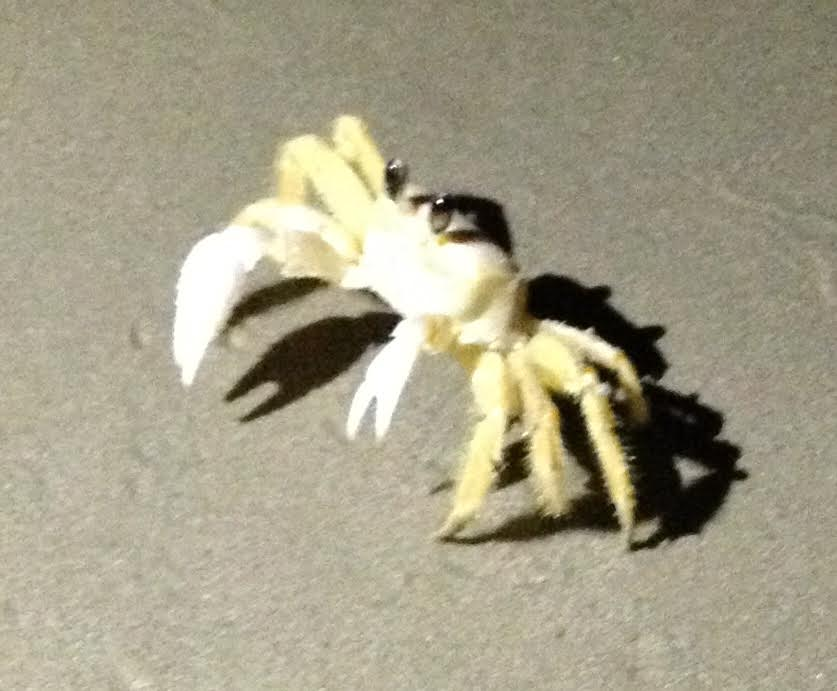
\includegraphics[
    width=0.6\textwidth]{Figures/crab.jpg}
    \caption{\label{fig:crab}Funny little crab}
    \label{fig:crab_label}
\end{figure}

Some words that mean nothing. Some words that mean nothing. Some words that mean nothing. Again, figure \ref{fig:crab} shows a funny little crab. Some words that mean nothing. Some words that mean nothing. Some words that mean nothing. Some words that mean nothing. Some words that mean nothing.

\subsection{Solution B}
Some words that mean nothing. Some words that mean nothing. Some words that mean nothing. Some words that mean nothing. Some words that mean nothing. Some words that mean nothing. Some words that mean nothing. Some words that mean nothing. Some words that mean nothing.

Some words that mean nothing. Some words that mean nothing. Some words that mean nothing. Some words that mean nothing. Some words that mean nothing. Some words that mean nothing. Some words that mean nothing. Some words that mean nothing. Some words that mean nothing.

Some words that mean nothing. Some words that mean nothing. Some words that mean nothing. Some words that mean nothing. Some words that mean nothing. Some words that mean nothing. Some words that mean nothing. Some words that mean nothing. Some words that mean nothing.

\subsection{Solution C}
Some words that mean nothing. Some words that mean nothing. Some words that mean nothing. Some words that mean nothing. Some words that mean nothing. Some words that mean nothing. Some words that mean nothing. Some words that mean nothing. Some words that mean nothing.

Some words that mean nothing. Some words that mean nothing. Some words that mean nothing. Some words that mean nothing. Some words that mean nothing. Some words that mean nothing. Some words that mean nothing. Some words that mean nothing. Some words that mean nothing.

Some words that mean nothing. Some words that mean nothing. Some words that mean nothing. Some words that mean nothing. Some words that mean nothing. Some words that mean nothing. Some words that mean nothing. Some words that mean nothing. Some words that mean nothing.

\section{Engineering analysis}
Engineering analysis and design with a discussion and demonstration of engineering judgment \ldots
Some words that mean nothing. Some words that mean nothing. Some words that mean nothing. Some words that mean nothing. Some words that mean nothing.

Some words that mean nothing. Some words that mean nothing. Some words that mean nothing. Some words that mean nothing. Some words that mean nothing. Some words that mean nothing. Some words that mean nothing. Some words that mean nothing. Some words that mean nothing.

Some words that mean nothing. Some words that mean nothing. Some words that mean nothing. Some words that mean nothing. Some words that mean nothing. Some words that mean nothing. Some words that mean nothing. Some words that mean nothing. Some words that mean nothing. {\textbf{Table \ref{tab:var_items} shows various items.}} Some words that mean nothing. Some words that mean nothing. Some words that mean nothing. Some words that mean nothing.

\begin{table}[!htbp]
    \centering
    \caption{Various items}
    \medskip
    \label{tab:var_items}
    \begin{tabular}{lrr} 
        %\toprule
        \hline
        \textbf{Item}   & \textbf{Qty}   & \textbf{Unit} \$   \\
        %\cmidrule
        \hline
        Widget & 1     & 199.99    \\
        Gadget & 2     & 399.99    \\
        Cable  & 3     & 19.99     \\
        %\bottomrule
        \hline
    \end{tabular}
\end{table}

\section{Conclusions}
From the analysis in the report body, it was concluded that \ldots 
Some words that mean nothing. Some words that mean nothing. Some words that mean nothing. Some words that mean nothing. Some words that mean nothing. Some words that mean nothing. Some words that mean nothing. Some words that mean nothing. Some words that mean nothing.

\section{Recommendations}
Based on the analysis and conclusions in this report, it is recommended that \ldots 
Some words that mean nothing. Some words that mean nothing. Some words that mean nothing. Some words that mean nothing. Some words that mean nothing. Some words that mean nothing. Some words that mean nothing. Some words that mean nothing. Some words that mean nothing.

% Back matter
\begin{singlespacing}
    
    \pagebreak
    \nocite{*}
    \bibliographystyle{IEEEtran}
    \renewcommand{\bibname}{\Large References}
    \bibliography{references}
    \addcontentsline{toc}{section}{References} % add to table of contents
    %\begin{thebibliography}{9}
    %\bibitem{lamport94}
    %    Leslie Lamport,
    %    \textit{\LaTeX: a document preparation system},
    %    Addison Wesley, Massachusetts,
    %    2nd edition,
    %    1994.
    %
    %\end{thebibliography}
    
    \pagebreak
    \section*{Glossary}
    \addcontentsline{toc}{section}{Glossary}
    
    \pagebreak
    \section*{Appendix A: Some Title}
    \addcontentsline{toc}{section}{Appendix A: Some Title}
    Some appendix worthy stuff to put into Appendix A, like tables of tedious data related to some discussion in the body of the report.
    
    \pagebreak
    \section*{Appendix B: Some Other Title}
    \addcontentsline{toc}{section}{Appendix B: Some Other Title}
    Some appendix worthy stuff to put into Appendix B, like tables of tedious data related to some discussion in the body of the report.
    
\end{singlespacing}

\end{document}

\usepackage[toc]{glossaries}
\makeglossaries
\newglossaryentry{computer}
{
  name=computer,
  description={is a programmable machine that receives input,
               stores and manipulates data, and provides
               output in a useful format}
}
\printglossaries